\documentclass{beamer}

\usepackage{beamerthemesplit}
\usetheme{Singapore} 
\usecolortheme{whale}

\input{../../include/preamble.inc} 
\input{../../include/definitions.inc} 
\input{../../include/author.inc} 

\title[]{Звуковые колебания}

\begin{document}
	
\frame[plain]{\titlepage}


\frame[plain]{
	\frametitle{Аннотация}
	\parbox{\textwidth}{
		Звуковые волны. Скорость звука (определение). Скорость звука в идеальном политропном газе. Линеаризация уравнений сохранения. Плоские и сферические звуковые волны. Запаздывающие потенциалы. Способы конструирования решений. Распространение возмущений с до- и сверхзвуковой скоростью. Монохромати\-чес\-кие волны и спектральное разложение. Волновой вектор и волновое число. Энергия и плотность потока энергии звуковых колебаний. Задача об отражении и преломлении звуковой волны.
	}
}

\frame{
	\frametitle{Основные уравнения динамики идеального газа}
	
	\begin{exampleblock}{Уравнения сохранения для идеального газа}
		\parbox{\textwidth}{
		\[
		\pd{\rho}{t} + (\vec{v} \cdot \nabla) \rho + \rho \divo \vec{v} = 0,
		\]
		\[
		\pd{\vec{v}}{t} + (\vec{v} \cdot \nabla) \vec{v} = -\frac{1}{\rho} \nabla p,
		\]
		\[
		\pd{S}{t} + (\vec{v} \cdot \nabla) S = 0.
		\]
			
		}
	\end{exampleblock}
	\begin{exampleblock}{Замыкающие соотношения}
		\parbox{\textwidth}{
			\[
			p = p(\rho, S)
			\]
		}
	\end{exampleblock}

}


\frame{
	\frametitle{Звуковые волны}
	
	\begin{exampleblock}{Определение}
		\parbox{\textwidth}{
			Колебательное движение с малыми амплитудами в сжимаемом газе называют \alert{звуковыми волнами}.
		}
	\end{exampleblock}\pause

	\begin{exampleblock}{Замечание}
		\parbox{\textwidth}{
			При рассмотрении звуковых колебаний будет считать течение \alert{изоэнтропическим} ($S=const$), тогда из общей системы уравнений остаются только уравнение неразрывности и уравнение Эйлера, а в замыкающем соотношении пропадает зависимость от $S$ как функции от координаты и времени.
		}
	\end{exampleblock}



	
}

\frame{
	\frametitle{Скорость звука}
		\begin{exampleblock}{Уравнения сохранения для идеального газа}
		\parbox{\textwidth}{
			\[
			\pd{\rho}{t} + \divo (\rho \vec{v}) = 0,\quad
			\pd{\vec{v}}{t} + (\vec{v} \cdot \nabla) \vec{v} = -\frac{1}{\rho} \left( \pd{p}{\rho} \right)_S \nabla \rho,
			\]
			\[
			p = p(\rho).
			\]
			
		}
	\end{exampleblock}\pause

	\begin{exampleblock}{Определение}
		\parbox{\textwidth}{
			Величина $c>0$, определяемая соотношением,
			\[
			c^2 = \left( \pd{p}{\rho} \right)_S,
			\]
			называется \alert{скоростью звука}. 
			
			\medskip
			Как видно из определения, $c = c(\rho, S)$. Для изоэнтропических течений зависимостью от $S$ как от функции переменных пространства и времени можно пренебречь.
		}
	\end{exampleblock}
	
}

\frame{
	\frametitle{Скорость звука в идеальном политропном газе}
	
	\parbox{\textwidth}{
	Уравнение состояние идеального политропного газа:
	\[
	p = A(S) \rho^\gamma\quad\text{или}\quad
	p = \rho R T / \mu,
	\]	
	где $\gamma=c_p/c_V$ -- показатель политропы, $A(S)$ -- функция энтропии, $p$~-- давление, $\rho$ -- плотность, $T$ -- температура, $R$ -- газовая постоянная, $\mu$ -- молярная масса газа.
	
	\[
	c^2 = \left(\pd{p}{\rho}\right)_S = \gamma A(S) \rho^{\gamma-1} = \frac{\gamma p}{\rho} =
	\gamma \frac{R T}{\mu}
	\]
	
	Таким образом,
	\[
		c = \sqrt{\gamma  \frac{R T}{\mu}}.
	\]
	}
	
	
}


\frame{
	\frametitle{Линеаризация уравнений движения}
	
	\begin{exampleblock}{Замена переменных}
		\parbox{\textwidth}{
			Рассмотрим малые колебания газа в окрестности постоянного решения 
			$\vec{v} = 0$, $p=p_0$, $\rho = \rho_0$:
			\[
			\begin{array}{lcl}
			\vec{v} & = & \vec{v},\\
			c  & = & c_0 + c',\\
			\rho & = & \rho_0 + \rho '.
			\end{array}
			\]
		}
	\end{exampleblock}\pause

	\begin{exampleblock}{Уравнения движения}
		\parbox{\textwidth}{
		\[
		\pd{(\rho_0 + \rho')}{t}+ \divo(\rho_0 + \rho') \vec{v} = 0,
		\]
		\[
		\pd{\vec{v}}{t} + (\vec{v} \cdot \nabla) \vec{v} = -\frac{1}{\rho_0+\rho'} (c_0 + c')^2 \nabla (\rho_0 + \rho').
		\]
		}
	\end{exampleblock}
	
	
}

\frame{
	\frametitle{Уравнения звуковых колебаний}
	
	\begin{exampleblock}{Основные уравнения}
		\parbox{\textwidth}{
			Считая колебания малыми, отбрасываем все слагаемые, имеющие порядок малости два и выше и получаем:
			\[
			\pd{\rho'}{t} + \rho_0 \divo \vec{v} = 0,\quad
			\pd{\vec{v}}{t} + \frac{c_0^2}{\rho_0} \nabla \rho' = 0.
			\]
		}
	\end{exampleblock}\pause

	\begin{exampleblock}{Потенциальное течение и волновое уравнение}
		\parbox{\textwidth}{
			Если $\vec{v} = \nabla \varphi$, тогда 
			\[
			\pd{\rho'}{t} + \rho_0 \Delta\varphi = 0,\quad
			\pd{}{t}\nabla\varphi + \frac{c_0^2}{\rho_0} \nabla \rho' = 0.
			\]
			\[
				\Downarrow
			\]
			\[
			\frac{1}{c_0^2} \pdk{\varphi}{t} = \Delta\varphi.
			\]
			
		}
	\end{exampleblock}
	
}

\frame{
	\frametitle{Решение волнового уравнения для плоских волн}
	
	\begin{exampleblock}{Одномерное плоское течение}
		\parbox{\textwidth}{
			Если $\varphi = \varphi(t,x)$, тогда решением полученного волнового уравнения будет:
			\[
			\varphi(t,x) = f_1(x - c_0 t) + f_2(x + c_0 t) = f_1(\xi) + f_2(\eta),
			\]
			где $f_1(\xi)$, $f_2(\eta)$ -- произвольные, дважды дифференцируемые функции своих аргументов
			\[
			\xi = x - c_0 t,\quad
			\eta = x + c_0 t.
			\]
		}
	\end{exampleblock}
	
}

\frame{
	\frametitle{ Прогрессивные волны }
	
	\begin{exampleblock}{}
		\centering
		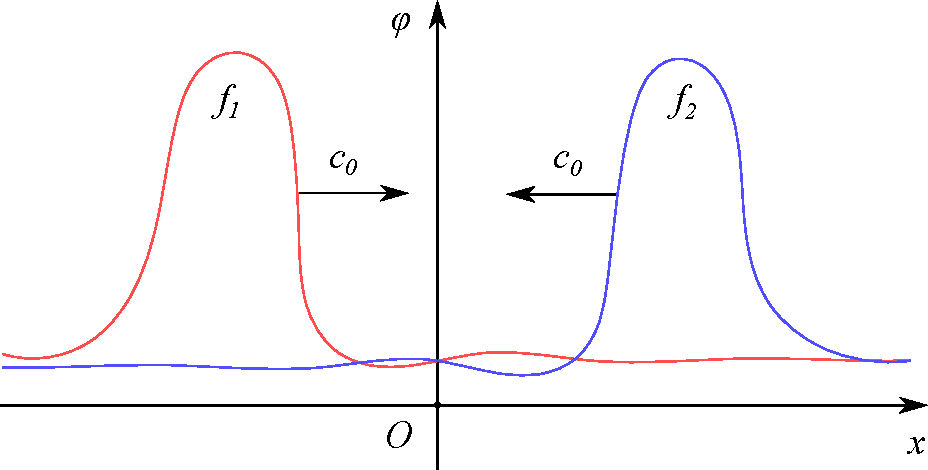
\includegraphics[width=0.9\linewidth]{../img/solitons.pdf}\\

		\parbox{\textwidth}{
			
			Решение $\varphi(t,x)$ представляет собой сумму перемещающихся пос\-тупательно вправо и влево волн неизменного вида со скоростью $c_0$
		}
	\end{exampleblock}
}


\foreach \n in {
	01, 02, 03, 04, 05, 06, 07}
{
	
	\frame{
		\frametitle{  Иллюстрация распространения плоских волн  }
		
		\centering
		\includegraphics[width=\linewidth]{../img/solitons/signal_\n.pdf}
		
		На рисунке $\varphi(t,x) =  f_1(x - c_0 t) + f_2(x + c_0 t)$ для заданных функций $f_1(\xi)$  и $f_2(\eta)$
	}
	
}

\frame{
	\frametitle{Решение волнового уравнения в сферической симметрии }
	
	\begin{exampleblock}{Волновое уравнение в сферической симметрии }
		\parbox{\textwidth}{
			Если $\varphi = \varphi(t,r)$, тогда волновое уравнение имеет вид:
			\[
			\frac{1}{c_0^2} \pdk{\varphi}{t} = \frac{1}{r^2}
			\left(
			\pd{}{r} 
			\left(
			r^2 \pd{\varphi}{r}
			\right)
			\right)\quad
			\iff\quad
			\frac{1}{c_0^2} \pdk{}{t} (r \varphi)= \pdk{}{r}
			\left(
			r \varphi
			\right).
			\]			
		}
	\end{exampleblock}
	
	\begin{exampleblock}{Одномерное сферическое течение}
		\parbox{\textwidth}{
			Решением полученного волнового уравнения будет:
			\[
			\varphi(t,r) = \frac{f_1(r - c_0 t) + f_2(r + c_0 t)}{r} = \frac{Q_1(\xi)}{r} + \frac{Q_2(\eta)}{r},
			\]
			где $Q_1(\xi)$, $Q_2(\eta)$ -- произвольные, дважды дифференцируемые функции своих аргументов
			$\xi = r - c_0 t$, $\eta = r + c_0 t$.
		}
	\end{exampleblock}
	
}

\foreach \n in {05, 06, 07, 08, 09, 10, 11, 12, 13, 14}
{
	
	\frame{
		\frametitle{  Иллюстрация распространения сферических волн }
		
		\centering
		\includegraphics[width=\linewidth]{../img/solitons/spherical_signal_\n.pdf}
		
		На рисунке $\varphi(t,r) = \displaystyle\frac{1}{r}\left( f_1(r - c_0 t) + f_2(r + c_0 t)\right)$ для заданных функций $f_1(\xi)$  и $f_2(\eta)$
		
	}
	
}


\frame{
	\frametitle{Запаздывающие потенциалы}
	
	\begin{exampleblock}{Определение}
		\parbox{\textwidth}{
			Возмущения из точки $r=0$ доходят до некоторой точки $r \neq 0$ только через определенное время, поэтому полученное решение волнового уравнения называется \alert{запаздывающим потенциалом}.
		}
	\end{exampleblock}\pause

	\begin{exampleblock}{Потенциал источника звука}
		\parbox{\textwidth}{
			Функция вида 
			\[
			\varphi^*(t,x,y,z) = 
			-\frac{Q
				\left(
					c_0(t-t_0) - \sqrt{(x-x_0)^2 + (y-y_0)^2 + (z-z_0)^2}
				\right) 
			}
			{4\pi \sqrt{(x-x_0)^2 + (y-y_0)^2 + (z-z_0)^2} }
			\]
			является решением волнового уравнения для источника звука, начинающего действовать в момент времени $t=t_0$ в точке с координатами $(x_0, y_0, z_0)$.
		}
	\end{exampleblock}
	
}

\frame{
	\frametitle{Способы конструирования решений волнового уравнения}
	
	\begin{exampleblock}{Принцип суперпозиций}
		\parbox{\textwidth}{
			В силу линейности волнового уравнения суммарным потенциалом при движении твердого тела по траектории 
			\[
			x_0 = x_0(t_0),\quad
			y_0 = y_0(t_0),\quad
			z_0 = z_0(t_0)
			\]
			можно рассматривать потенциал, являющийся суммой источников звука, возбуждаемых телом в момент времени $t_0$ в соответствующих точках траектории с заданной интенсивностью $Q_{t_0}$, при этом
			\[
			\varphi = \int\limits_0^t \varphi^* dt_0.
			\]
			
		}
	\end{exampleblock}
	
}


\frame{
	\frametitle{ Распространение возмущений от источника, движущегося с дозвуковой скоростью }
	\begin{columns}
		\begin{column}{0.5\textwidth}
			\centering
				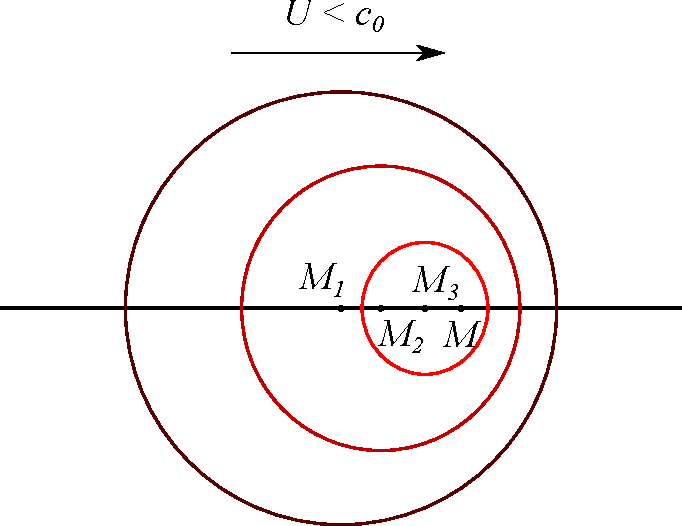
\includegraphics[width=\linewidth]{../img/under_sonic}
		\end{column}
		\begin{column}{0.5\textwidth}
			\parbox{\textwidth}{
				При движении тела прямолинейно с дозвуковой скоростью
				\[
				U < c_0
				\]
				возмущения, возникающие на траектории его движения, движутся быстрее, чем само тело, поэтому в его окрестности среда до него и после \alert{возмущена}. Возмущения, посланные источником звука ранее, всегда обгоняют более поздние.
			}
			
		\end{column}
	\end{columns}

}

\frame{
	\frametitle{ Распространение возмущений от источника, движущегося с дозвуковой скоростью }
	\begin{columns}
		\begin{column}{0.5\textwidth}
			\centering
			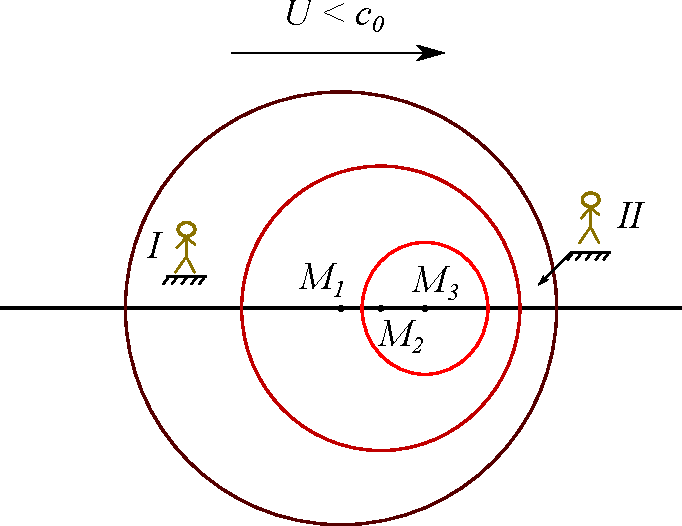
\includegraphics[width=\linewidth]{../img/under_sonic_doppler}
		\end{column}
		\begin{column}{0.5\textwidth}
			\begin{exampleblock}{Эффект Допплера}
				\parbox{\textwidth}{
					При движении тела прямолинейно с дозвуковой скоростью
					\[
					U < c_0
					\]
					частота звука перед телом (положение II) имеет большую частоту, чем за ним (положение I). Это обстоятельство объясняет так называемый \alert{эффект Допплера}.
				}
			\end{exampleblock}
		\end{column}
	\end{columns}
	
}

\frame{
	\frametitle{ Распространение возмущений от источника, движущегося со сверхзвуковой скоростью }
	\begin{columns}
		\begin{column}{0.5\textwidth}
			\centering
			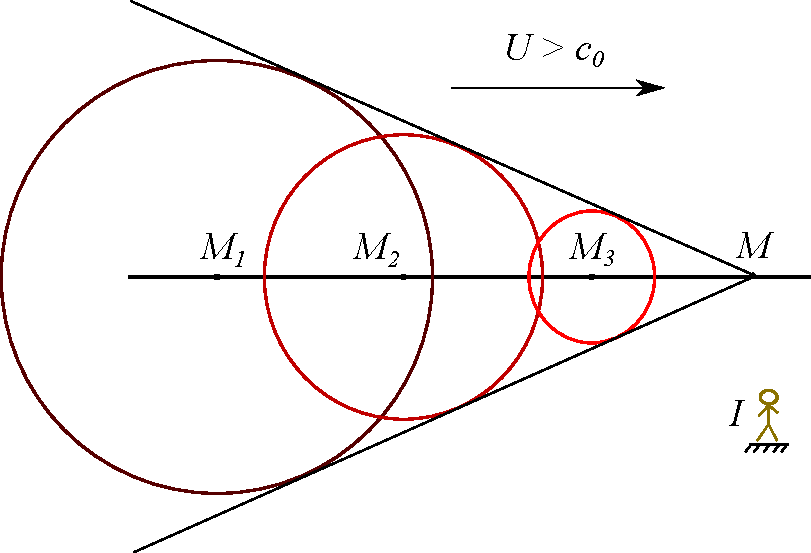
\includegraphics[width=\linewidth]{../img/super_sonic}
		\end{column}
		\begin{column}{0.5\textwidth}
%			\begin{exampleblock}{Эффект Допплера}
				\parbox{\textwidth}{
					При движении тела прямолинейно со сверхзвуковой скоростью
					\[
					U > c_0
					\]
					возмущения от источника будут распространяться медленнее, чем тело. Поэтому среда перед телом всегда будет \alert{невозмущенная}. Наблюдатель, стоящий перед источником, движущимся со сверхзвуковой скоростью, \alert{не слышит} звуковых колебаний, создаваемых этим источником.
					
				}
%			\end{exampleblock}
		\end{column}
	\end{columns}
	
}

\frame{
	\frametitle{ Распространение возмущений от источника, движущегося со сверхзвуковой скоростью }
	\begin{columns}
		\begin{column}{0.5\textwidth}
			\centering
			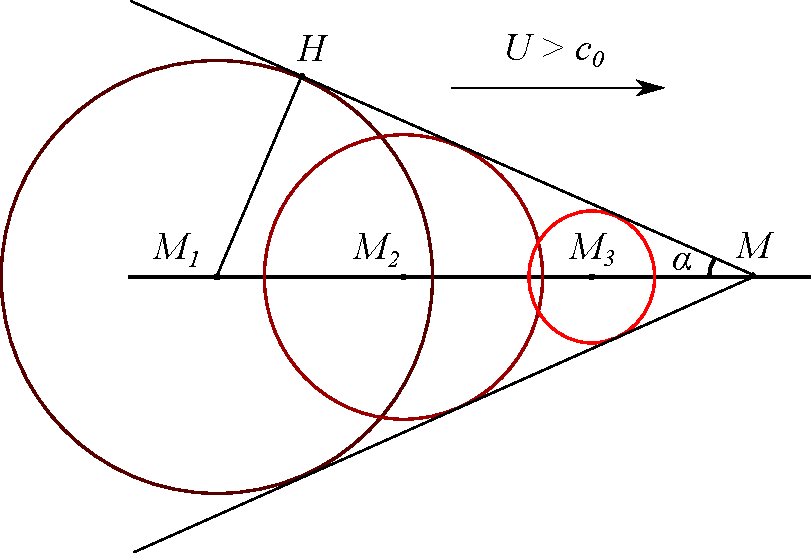
\includegraphics[width=\linewidth]{../img/Mach_cone}
		\end{column}
		\begin{column}{0.5\textwidth}
			\begin{exampleblock}{Конус Маха}
			\parbox{\textwidth}{
				При движения тела прямолинейно со сверхзвуковой скоростью
				$U > c_0$ огибающая возмущений будет образовывать конус с углом при вершине $\angle HMM_1$, обозначенным $\alpha$, таким, что

			}
			\end{exampleblock}
		\end{column}
	\end{columns}

	\parbox{\textwidth}{
	\[
	\sin\alpha = \frac{M_1H}{M_1M} = \frac{c_0 \Delta t}{U \Delta t} = \frac{c_0}{U} = \frac{1}{M},
	\]
	где $\Delta t$ -- время, за которое тело прошло расстояние $M_1M$; $M=U/c_0$ -- \alert{число Маха}.	
	
	\medskip
	Угол $\alpha$ называется \alert{углом Маха}, а поверхность конуса -- \alert{конусом Маха}.
	}
	
	
}


\frame{
	\frametitle{Монохроматические волны}
	
	\begin{exampleblock}{Определение}
		\parbox{\textwidth}{
			\alert{Монохроматической волной} называют функции, в которых все величины являются простыми периодическим (гармоническими) функциями времени вида:
			\[
			\varphi_0 = \Re \{ \varphi_0(x,y,z) e^{-i\omega t}  \},
			\]
			где $\omega$ -- частота волны.
		}
	\end{exampleblock}

	\begin{exampleblock}{Уравнение монохроматической волны}
		\parbox{\textwidth}{
			\[
			\Delta \varphi_0 + \frac{\omega^2}{c^2}\varphi_0 = 0
			\]
			Уравнение получается с помощью подстановки выражения для монохроматической волны в волновое уравнение.
		}
	\end{exampleblock}
	
}

\frame{
	\frametitle{Бегущая плоская монохроматическая волна}
	\begin{exampleblock}{Определение}
		\parbox{\textwidth}{
			Потенциал вида
			\[
			\varphi = \Re \left\{ 
			A e^{-i \omega \left( t - \frac{x}{c}\right)}
			\right\}
			\]
			является бегущей плоской монохроматической волной, где $A$ -- комплексная амплитуда. 
		}
	\end{exampleblock}
	\begin{exampleblock}{Вещественное представление}
		\parbox{\textwidth}{
		\[
		\varphi = a \cos \left(
		\frac{\omega}{c} x - \omega t + \alpha
		\right),
		\]
		где $a$ -- вещественная амплитуда волны, аргумент под знаком $\cos$ -- фаза.
		}
	\end{exampleblock}
}

\frame{
	\frametitle{Волновой вектор и волновое число}
	\begin{exampleblock}{Определение}
		\parbox{\textwidth}{
			Вектор 
			\[
			\vec{k} = \frac{\omega}{c}\vec{n} = \frac{2\pi}{\lambda}\vec{n}
			\]
			называют \alert{волновым вектором}, а его абсолютную величину~-- \alert{волновым числом}, где $\vec{n}$ -- единичный вектор в направлении расп\-рост\-ранения волны. 
		}
	\end{exampleblock}

	\begin{exampleblock}{Спектральное разложение}
		\parbox{\textwidth}{
			Вообще, любую волну можно представить в виде совокупности плоских монохроматических волн с различными волновыми векторами и частотами вида:
			\[
			\varphi = \Re \left\{
				A e^{i(\vec{k}\cdot\vec{r} - \omega t)} 
				\right\},
			\]
			где $\vec{r}$ -- радиус вектор. Такое разложение является разложением в ряд, или интегралом Фурье. 
		}
	\end{exampleblock}
}


\frame{
	\frametitle{Энергия звуковых колебаний}
	
	\begin{exampleblock}{Закон сохранения энергии идеального газа}
		\parbox{\textwidth}{
			\[
			\pd{}{t}\rho \left(\varepsilon + \frac{v^2}{2} \right) + 
			\divo \rho\vec{v}\left(\varepsilon + \frac{v^2}{2} + \frac{p}{\rho}\right) = 0
			\]
			
		}
	\end{exampleblock}
	
	\begin{exampleblock}{Энергия единицы объема}
		\parbox{\textwidth}{
			Разложение полной энергии единицы объема покоящейся сплошной среды относительно состояния $\rho_0$, $\varepsilon_0$ при ее малых возмущениях
			\[
			\rho = \rho_0 + \rho',\quad
			\varepsilon = \varepsilon_0 + \varepsilon'
			\]
			до второго порядка малости имеет вид:
			\[
			E = \rho\varepsilon+\frac{\rho v^2}{2} \approx
			\rho_0 \varepsilon_0 + \rho' \left. \pd{(\rho\varepsilon)}{\rho} \right|_{\rho=\rho_0} + \left.\frac{\rho'^2}{2} \pdk{(\rho\varepsilon)}{\rho} \right|_{\rho=\rho_0}+ \frac{\rho_0 v^2}{2}.
			\]
			
		}
	\end{exampleblock}
	
}

\frame{
	\frametitle{Энергия звуковых колебаний}
	
	\begin{exampleblock}{Термодинамические соотношения}
		\parbox{\textwidth}{
			Так как
			\[
			d\varepsilon = T dS - p dV = T dS + \frac{p}{\rho^2} d\rho
			\quad\text{или}\quad
			dw = T dS + \frac{dp}{\rho},
			\]
			где $w = \varepsilon + p/\rho$ -- энтальпия,	то
			\[
			\left( \pd{(\rho\varepsilon)}{\rho}  \right)_S = \varepsilon + \frac{p}{\rho} = w,
			\]\pause
			\[
			\left( \pdk{(\rho\varepsilon)}{\rho} \right)_S = 
			\left( \pd{w}{\rho} \right)_S = \left( \pd{w}{p} \right)_S \left( \pd{p}{\rho} \right)_S = \frac{c^2}{\rho}.
			\]
		}
	\end{exampleblock}
	
}


\frame{
	\frametitle{ Энергия звуковых колебаний}
	
	\begin{exampleblock}{Полная энергия единицы объема сплошной среды}
		\parbox{\textwidth}{
			\[
				E \approx \rho_0 \varepsilon_0 + w_0 \rho' + \frac{c_0^2}{2\rho_0}\rho'^2 + \rho_0 \frac{v^2}{2},
			\]\pause
			где
			\begin{enumerate}[label = \arabic*)]
				\item $\rho_0 \varepsilon_0$ -- энергия единицы объема неподвижной среды;\pause
				\item $w_0 \rho'$ -- изменение энергии, связанное с изменением количества вещества (массы).
			\end{enumerate}
		}
	\end{exampleblock}\pause

	\begin{exampleblock}{Плотность звуковой энергии}
		\parbox{\textwidth}{
			\[
			E_s = \frac{\rho_0 v^2}{2} + \frac{c_0^2 \rho'^2}{2\rho_0}
			\]\pause
			
			В случае плоских волн $\rho' = \rho_0 v/c_0$:
			\[
			E_s = \rho_0 v^2.
			\]
			
		}
	\end{exampleblock}

	

	
}

\frame{
	\frametitle{ Плотность потока энергии звуковых колебаний }
	
	\begin{exampleblock}{Плотность потока энергии}
		\parbox{\textwidth}{
			Линеаризация плотности потока покоящегося идеального газа около состояния
			\[
				w = w_0 + w',\quad p = p_0 + p'
			\]
			имеет вид:
			\[
			\vec{j} = \rho\vec{v} \left(\varepsilon + \frac{v^2}{2} + \frac{p}{\rho}\right) =
			\rho\vec{v} \left(\frac{v^2}{2} + w \right) \approx
			w_0 \rho \vec{v} + \rho w' \vec{v}.
			\]
		}
	\end{exampleblock}


}

\frame{
	\frametitle{Плотность потока энергии звуковых колебаний}
	\small
	\begin{exampleblock}{}
		\parbox{\textwidth}{
			С точностью до первого порядка малости
			$w' = \left( \displaystyle\pd{w}{p} \right)_S p' = \displaystyle\frac{p'}{\rho}$, отсюда:
			\[
			\vec{j} \approx w_0 \rho \vec{v} + p'\vec{v},
			\]\pause
			где слагаемое $w_0 \rho \vec{v}$ отвечает за плотность потока энергии, связанного с движением массы.
		}
	\end{exampleblock}\pause
	\begin{exampleblock}{Плотность потока энергии звуковых колебаний}
		\parbox{\textwidth}{
		\[
		\vec{j}_s = p'\vec{v}
		\]	
		}
	\end{exampleblock}\pause
	\begin{exampleblock}{Плоская волна}
	\parbox{\textwidth}{
		Учитывая соотношение для плоской волны $p' = c_0 \rho_0 v$,  получим:
		\[
		\vec{j}_s = c_0 \rho_0 v^2 \vec{n} = c_0 E_s \vec{n},
		\]
		где $\vec{n}$ -- вектор направления движения волны, $E_s$ -- энергия плоской звуковой волны.
	}
	\end{exampleblock}
}


\frame{
	\frametitle{Уравнение сохранения энергии для звуковых колебаний }
				\[
	\pd{E_s}{t} + \divo \vec{j}_s = 0,
	\]
	где
	\[
	E_s = \frac{\rho_0 v^2}{2} + \frac{c_0^2 \rho'^2}{2\rho_0},
	\]
	\[
	\vec{j}_s = p'\vec{v}.
	\]
}


\frame{
	\frametitle{ Задача об отражении и преломлении волны }
	
	\centering
	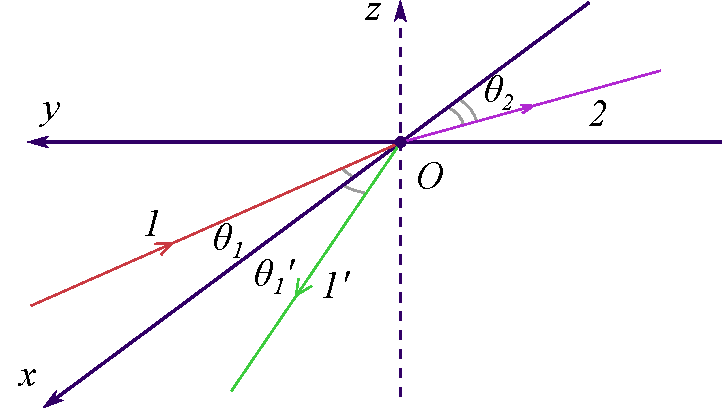
\includegraphics[width=0.6\linewidth]{../img/sonic_waves_reflection.pdf}
	

	\only<1>{
	\begin{exampleblock}{Постановка задачи}
		\parbox{\textwidth}{
			Описать отраженную и преломленную волны, получившиеся в результате взаимодействия падающей монохроматической волны с границей раздела двух сред.
		}
	\end{exampleblock}
	}
	\only<2>{
	\begin{exampleblock}{Основные предположения}
		\parbox{\textwidth}{
		Волна падает в плоскости Oxy, а граница раздела находится в плоскости  Oxz.
		}
	\end{exampleblock}
	}

	\only<3>{
	\begin{exampleblock}{Основные предположения}
		\parbox{\textwidth}{
			Все три волны будут иметь одинаковые частоты $\omega$ и одинаковые компоненты $k_y$, $k_z$, т.к. уравнение, описывающее волну одно и то же, а граничные условия при $x=0$ не зависят от $y$, $z$, $\omega$.
		}
	\end{exampleblock}
	}

	\only<4>{
	\begin{exampleblock}{Волновые векторы}
		\parbox{\textwidth}{
			Из рисунка видно, что
			\[
			\vec{k}_1 = \frac{\omega}{c_1}(-\cos\theta_1; -\sin\theta_1; 0),\quad
			\vec{k}_1' = \frac{\omega}{c_1}(\cos\theta_1'; -\sin\theta_1'; 0),
			\]
			\[
			\vec{k}_2 = \frac{\omega}{c_2}(-\cos\theta_2; -\sin\theta_2; 0).
			\]
			
		}
	\end{exampleblock}
	}

	\only<5>{
	\begin{exampleblock}{Граничные условия}
		\parbox{\textwidth}{
			Из того, что $k_y$ одно и то же во всех трех волнах, следует, что
			\[
			\theta_1 = \theta_1'
			\quad\text{и}\quad
			\frac{\sin\theta_1}{\sin\theta_2} = \frac{c_1}{c_2}.
			\]
			
		}
	\end{exampleblock}
	}

	\only<6>{
	\begin{exampleblock}{Потенциалы волн}
		\parbox{\textwidth}{
			
		\[
		\varphi_1 = A_1 \exp \left\{ 
		i\omega\left(
		-\frac{x}{c_1}\cos\theta_1 - \frac{y}{c_1}\cos\theta_1 -t 
		\right)
		 \right\},
		\]
		\[
		\varphi_1' = A_1' \exp \left\{ 
		i\omega\left(
		\frac{x}{c_1}\cos\theta_1 - \frac{y}{c_1}\cos\theta_1 -t 
		\right)
		\right\},
		\]
		\[
		\varphi_2 = A_2 \exp \left\{ 
		i\omega\left(
		-\frac{x}{c_2}\cos\theta_2 - \frac{y}{c_2}\cos\theta_2 -t 
		\right)
		\right\}.
		\]
		
		}
	\end{exampleblock}
	}


	\only<7>{
	\begin{exampleblock}{Граничные условия}
		\parbox{\textwidth}{
			Из условий сохранения на контактном разрыве следует равенство давления ($p = -\rho (\partial\varphi/\partial t)$) и непрерывность нормальной составляющей скорости ($v_x = \partial \varphi / \partial x$):
			\[
			\rho_1(A_1 + A_1') = \rho_2 A_2,\quad
			\frac{\cos\theta_1}{c_1}(A_1 - A_1') = 
			\frac{\cos\theta_2}{c_2} A_2.
			\]
			
		}
	\end{exampleblock}
	}

	\only<8>{
	\begin{exampleblock}{Коэффициент отражения}
		\parbox{\textwidth}{
			Коэффициент отражения определяет отношение средних  (по времени) плотностей потока энергии в отраженной и падающей волнах:
			\[
				R = \frac{c_1\rho_1 \overline{v_1'^2} }{ c_1\rho_1 \overline{v_1^2}} =
				\frac{|A_1'|^2}{|A_1|^2} = 
				\left(
					\frac{\rho_2 \tg \theta_2 - \rho_1 \tg\theta_1}{\rho_2 \tg\theta_2 + \rho_1\tg\theta_1}
				\right)^2.
			\]
			
		}
	\end{exampleblock}
	}

	\only<9>{
		\begin{exampleblock}{Коэффициент отражения}
			\parbox{\textwidth}{
				\[
				R = 
				\left[
				\frac{\rho_2 c_2 \cos\theta_1 - \rho_1 \sqrt{c_1^2 - c_2^2 \sin^2\theta_1}}{\rho_2 c_2 \cos\theta_1 + \rho_1 \sqrt{c_1^2 - c_2^2 \sin^2\theta_1}}
				\right]^2
				\]
				
			}
		\end{exampleblock}
	}	

}





\frame{
	\frametitle{ Литература }
	\begin{literature} %[partopsep=1pt,label=\textbullet]


		\item {\em Ландау~Л.\,Д., Лифшиц~Е.\,М.} Теоретическая физика: Учебное пособие. В 10 т. Т. VI. Гидродинамика. -- 3-е изд., перераб. --- М.: Наука. Гл. ред. физ-мат. лит., 1986.

		\item {\em Седов Л.\,И.} 
		Механика сплошной среды. Том 2. М.:Наука, 1970.

	\end{literature}
}



\end{document}